\documentclass[10pt,a4paper]{article}

\usepackage[latin1]{inputenc}
\usepackage{amsmath}
\usepackage{amsfonts}
\usepackage{amssymb}
\usepackage{graphicx}
\usepackage{listings}
\title{Assignment No :A3}
\date{}
\author{Roll No.4431}


\begin{document}
\maketitle
\section{Title:}
Message Passing Interface (MPI) for coverage.

\section{Problem Definition}
Write a MPI program for calculating a quantity called coverage from data files.
Hint :- Program distributes computation efficiently across the cluster. The program should be able to
work with any number of nodes and should yield the same results as the serial code.

\section{Learning Objectives}
\begin{enumerate}
\item To understand the concept Message Passing Interface in parallel programming.
\item To understand applications of MPI in real world.
\item To be able to solve the coverage problem.
\end{enumerate}

\section{Learning Outcomes}
\begin{enumerate}
\item Ability to analyze problems and induce MPI based parallelism in them properly.
\item Understanding of parallel/concurrent programming.\end{enumerate}


\section{Related Mathematics}
Let S be the solution perspective of the given problem.
\\\\The set S is defined as:
\\\\$S=\lbrace\ s,e,X,Y,F,DD,NDD,S_{c},F_{c}|\varnothing_{s}\rbrace$
\\\\Where,
\\\\s= Start state,  Such that $Y=\lbrace \varnothing \rbrace$ 
\\\\e= End state 
\\\\X= Input Set.
\\\\$X=\lbrace$ seq(x) $\mid$ x $\in$ Natural numbers $\rbrace$
\\\\Y=Output set.
\\\\$Y=\lbrace Coverage Of The Sequence \rbrace $
\\\\F= Set of functions used.
\\\\F=$\lbrace master(), slave(), compute()\rbrace$
\\\\master()= function for master purposes.
\\\\slave()= function for slave purposes.
\\\\compute()= function for computing the coverage of the input sequence.
\\\\DD=Deterministic data.
\\DD=
\begin{enumerate}
\item sequence follows proper constraints.
\item coverage is defined and exists.
\item sequence terminates.
\end{enumerate}
NDD= Non-deterministic data.
\\NDD= $\cup$ - DD


\section{State Transition diagram}
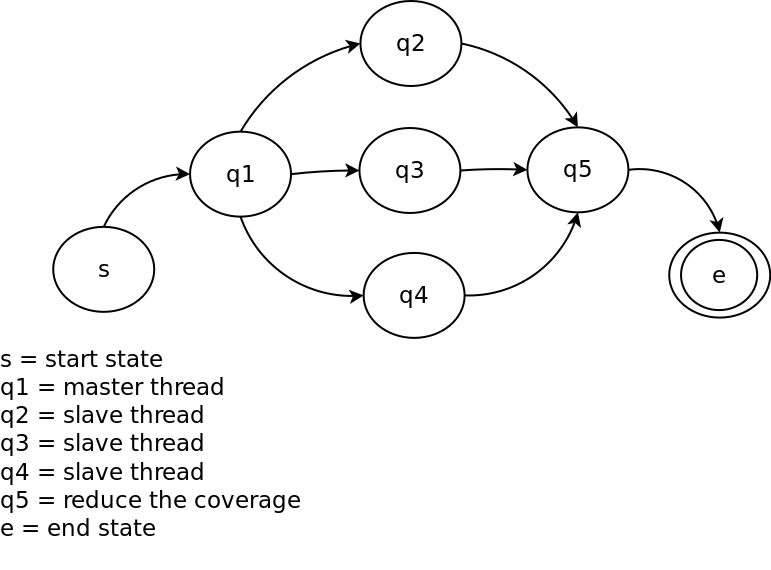
\includegraphics[scale=0.30]{stdg.png}

\section{Concepts related theory}
\subsection{Concept of MPI}
		\paragraph{} MPI is a specification for the developers and users of message passing libraries. By itself, it is NOT a library - but rather the specification of what such a library should be. 
		
		MPI primarily addresses the message-passing parallel programming model: data is moved from the address space of one process to that of another process through cooperative operations on each process. 	 
		Simply stated, the goal of the Message Passing Interface is to provide a widely used standard for writing message passing programs. 
		
		The Message Passing Interface Standard (MPI) is a message passing library standard based on the consensus of the MPI Forum, which has over 40 participating organizations, including vendors, researchers, software library developers, and users. 	 
		The goal of the Message Passing Interface is to establish a portable, efficient, and flexible standard for message passing that will be widely used for writing message passing programs. MPI is not an IEEE or ISO standard, but has in fact, become the "industry standard" for writing message passing programs on HPC platforms. 
	
		
\subsection{MPI Programming Model:}	

		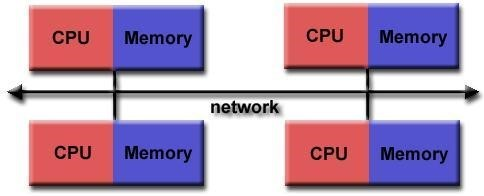
\includegraphics{MPI_01}

		  
		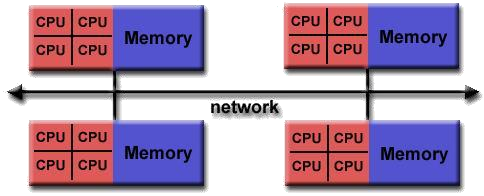
\includegraphics{MPI_02}
		\\
		\\
		Both the diagrams show the general programming model of the 
		MPI \\ system.
		
		

	\subsection{General MPI Programming Structure}
		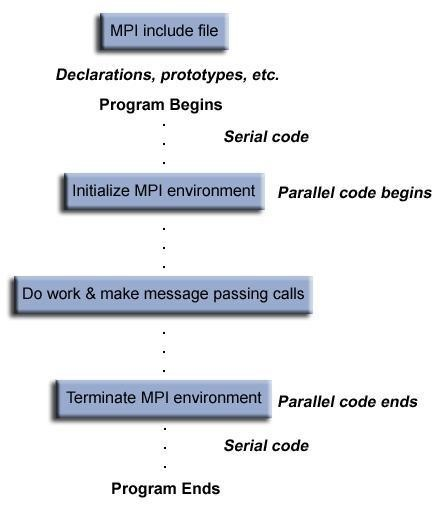
\includegraphics[width=\textwidth]{MPI_03}
\newpage		
\textbf{Communicators and Groups:} \\ \\
MPI uses objects called communicators and groups to define which collection of processes may communicate with each other.\\ \\
Most MPI routines require you to specify a communicator as an argument.\\ \\ 
MPI\_COMM\_WORLD whenever a communicator is required - it is the predefined communicator that includes all of your MPI processes. \\ \\

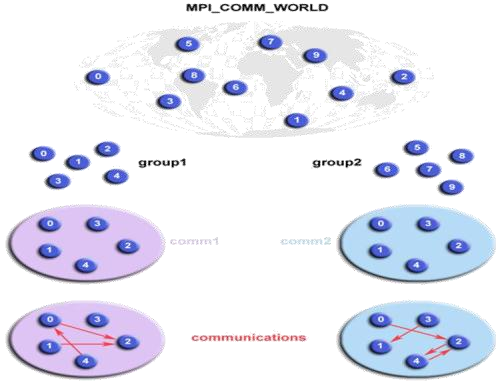
\includegraphics{MPI_04.png}
\newpage

\textbf{Level of Thread Support:} \\ 
MPI libraries vary in their level of thread support: \\
\begin{itemize}
	\item	MPI\_THREAD\_SINGLE - Level 0: Only one thread will execute.  
	\item	MPI\_THREAD\_FUNNELED - Level 1: The process may be multi-threaded, but only the main thread will make MPI calls - all MPI calls are funneled to the main  thread.  
	\item	MPI\_THREAD\_SERIALIZED - Level 2: The process may be multi-threaded, and multiple threads may make MPI calls, but only one at a time. That is, calls are 
	not made concurrently from two distinct threads as all MPI calls are serialized.  
	\item	MPI\_THREAD\_MULTIPLE - Level 3: Multiple threads may call MPI with no restrictions.
\end{itemize}	 
  
\textbf{Pros of MPI:} 
\begin{itemize}
	\item  runs on either shared or distributed memory architectures 
	\item  can be used on a wider range of problems than OpenMP 
	\item  each process has its own local variables 
	\item distributed memory computers are less expensive than large shared memory computers 
\end{itemize} 
 
\textbf{Cons of MPI:}  
\begin{itemize}
	\item requires more programming changes to go from serial to parallel version O can be harder to debug 
	\item  performance is limited by the communcation network between the nodes 
	
\end{itemize}

\newpage

\section{MPI Scatter, Gather:} 

MPI\_Gather( void* send\_data, int send\_count,  MPI\_Datatype send\_datatype, void* recv\_data, int recv\_count, MPI\_Datatype recv\_datatype,  	int root, MPI\_Comm communicator) \\ \\
MPI\_Bcast( void* data,  int count,  MPI\_Datatype datatype,  int root, MPI\_Comm communicator)

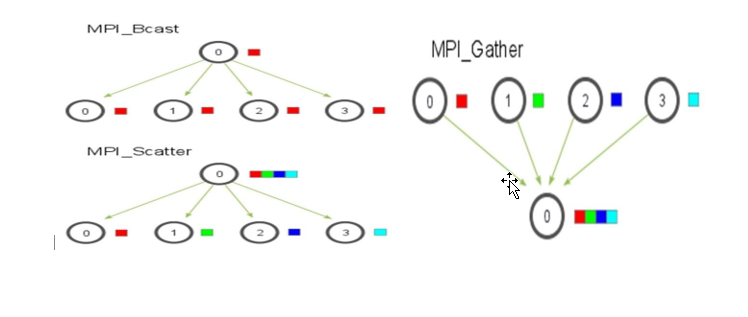
\includegraphics[scale=0.75]{MPI_06}

\section{Program Listing}
\begin{lstlisting}
// Assignment No 3(Coverage)

#include <stdio.h>
#include <stdlib.h>
#include <mpi.h>
#define v 1 /* verbose flag, output if 1, no output if 0 */
#define tag 100 /* tag for sending a number */
int main ( int argc, char *argv[] )
{
int p,myid,i,f,*x;
double start, end;
MPI_Status status;
MPI_Init(&argc,&argv);
MPI_Comm_size(MPI_COMM_WORLD,&p);
MPI_Comm_rank(MPI_COMM_WORLD,&myid);
if(myid == 0) /* the manager allocates and initializes x */
{
x = (int*)calloc(p,sizeof(int));
x[0] = 50;
for (i=1; i<p; i++) x[i] = 2*x[i-1];
if(v>0)
{
printf("The data to square : ");
for (i=0; i<p; i++)
 printf(" %d",x[i]);
 printf("\n");
}
}
if(myid == 0) /* the manager copies x[0] to f */
{             /* and sends the i-th element to the i-th processor */
f = x[0];
for(i=1; i<p; i++) 
MPI_Send(&x[i],1,MPI_INT,i,tag,MPI_COMM_WORLD);
}
else /* every worker receives its f from root */
{
MPI_Recv(&f,1,MPI_INT,0,tag,MPI_COMM_WORLD,&status);
if(v>0) 
printf("Node %d will square %d\n",myid,f);
}
start = MPI_Wtime();
f *= f;       /* every node does the squaring */
if(myid == 0) /* the manager receives f in x[i] from processor i */
for(i=1; i<p; i++)
MPI_Recv(&x[i],1,MPI_INT,i,tag,MPI_COMM_WORLD,&status);
else     /* every worker sends f to the manager */
MPI_Send(&f,1,MPI_INT,0,tag,MPI_COMM_WORLD);
if(myid == 0) /* the manager prints results */
{
x[0] = f;
printf("The squared numbers : ");
for(i=0; i<p; i++) 
printf(" %d",x[i]);
 printf("\n");
end = MPI_Wtime();
printf("Runtime = %f\n", end-start);
}

MPI_Finalize();
return 0;
}
\end{lstlisting}


\section{Output}
\begin{lstlisting}
botman@botmatrix:~$ mpicc Square_MPI1.c -o abc
botman@botmatrix:~$ mpirun -np 2 ./abc
The data to cover :  50 100
The covered numbers :  2500 10000
Runtime = 0.000311
Node 1 will cover 100
botman@botmatrix:~$ 


\end{lstlisting}

\section{TESTING :}
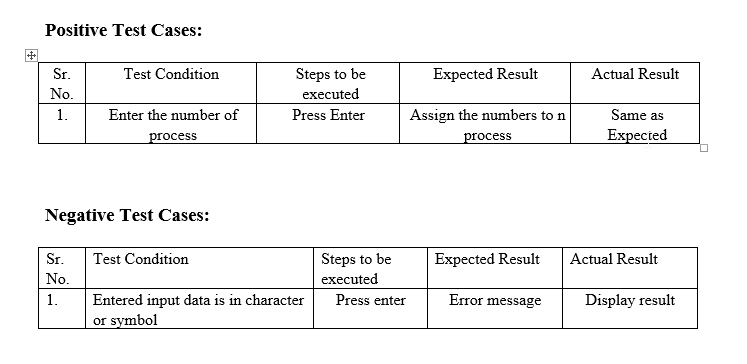
\includegraphics[scale=0.75]{MPI_07}

			
\section{CONCLUSION : }
	Thus, we have implemented a MPI Program for calculating a quantity called coverage from data files.

\end{document}